\documentclass[]{article}

\usepackage{amsmath}
\usepackage{amsfonts}
\usepackage{amssymb}

\usepackage[]{algorithm2e}

\usepackage{booktabs}
\usepackage{rotating}

%%% for dags
\usepackage{tikz}
\usetikzlibrary{arrows}
\usetikzlibrary{fit,positioning, backgrounds}

%%% BibTex packages (url for website references)
\usepackage[english]{babel}
\usepackage[round]{natbib}

%opening
\title{Consensus clustering for Bayesian mixture models: Supplementary materials}
\author{Stephen Coleman, Paul DW Kirk\, and Chris Wallace}

\begin{document}

\maketitle

\begin{abstract}

\end{abstract}

\section{Yeast data}

The "Yeast data" consists of three \emph{S. cerevisiae} datasets with gene products associated with a common set of 551 genes. The datasets are:
\begin{itemize}
	\item microarray profiles of RNA expression from \cite{granovskaia2010high}. This a cell cycle dataset that comprises measurements taken at 41 time points (the \textbf{Timecourse} dataset).
	\item Chromatin immunoprecipitation followed by microarray hybridization (\textbf{ChIP-chip}) data from \cite{harbison2004transcriptional}. This dataset has 117 features.
	\item Protein-protein interaction (\textbf{PPI}) data from BioGrid \citep{stark2006biogrid}. This dataset has 603 features.
\end{itemize}
The datasets were reduced to 551 items by considering only the genes identified by \cite{granovskaia2010high} as having periodic expression profiles with no missing data in the PPI and ChIP-chip data, following the same steps as the original MDI paper \citep{kirk2012bayesian}. The datasets were modelled using a base measure of a Gaussian process in the Timecourse dataset and Multinomial distributions in the ChIP-chip and PPI datasets.

\subsection{Bayesian analysis} \label{sec:bayesianAnalysis}
10 chains were run for 36 hours, resulting in 676,000 iterations per chain, thinned to every thousandth sample, resulting in 676 samples per chain. 

\subsubsection{Convergence} \label{sec:bayesianConvergence}
These chains were investigated for 
\begin{itemize}
	\item within-chain stationarity using the Geweke convergence diagnostic \citep{geweke1991evaluating}, and
	\item across-chain convergence using the potential scale reduction factor \citep[$\hat{R}$, ][]{gelman1992inference} and the Vats-Knudson extension \citep[\emph{stable $\hat{R}$},][]{vats2018revisiting}.
\end{itemize}
The Geweke convergence diagnostic is a standard Z-score; it compares the sample mean of two sets of samples (in this case buckets of samples from the first half of the samples to the sample mean of the entire second half of samples). It is calculated under the assumption that the two parts of the chain are asymptotically independent and if this assumption holds than the scores are expected to be standard normally distributed presenting evidence for within chain stationarity.

$\hat{R}$ is expected to approach 1.0 if the set of chains are converged. Low $\hat{R}$ is not sufficient in itself to claim chain convergence, but values above 1.1 are clear evidence for a lack of convergence \citep{gelman2013bayesian}. \cite{vats2018revisiting} show that this threshold is significantly too high (1.01 being a better choice) and propose extensions to $\hat{R}$ that enable a more formal rule for a threshold. It is their method as implemented in the R package \texttt{stableGR} \citep{knudson20202stableGR} that is the final check of convergence.

We focus upon stationarity of the continuous variables. This is as convergence of the allocation labels is difficult due to the label-switching problem. In MDI, the continuous variables consist of the concentration parameters of the Dirichlet distribution for the dataset-specific component weights and the $\phi_{ij}$ parameter associated with the correlation between the $i^{th}$ and $j^{th}$ datasets. 

We plot the Geweke-statistic for each chain in figure \ref{fig:gewekePlot} and the series of the $\phi$ parameters alone in figure \ref{fig:gewekePhiPlot}, excluding the most poorly behaved chain (chain 9). Very few of the chains appear to be truly stationary, but some behave far worse than others. Based upon this we exclude chains 1, 2, 4, 6 and 9, restricting the analysis to the 5 better, if not ideally, behaved chains. Further evidence that even these chains are not converged can be see in figure \ref{fig:gelmanPlot}, where the values of $\hat{R}$ do not drop below 1.25 for the $\phi$ parameters. Stable $\hat{R}$ is also too high, with several million more samples recommended before convergence is expected.

Investigating the Posterior similarity matrices (PSMs) we can see that the Timecourse data appears to have only the mildest of disagreement between the PSMs from different chains. The lack of convergence between chains emerges in the ChIP-chip data and, to a far greater degree, in the PPI data.

\begin{figure}
	\centering
	\includegraphics[scale=1.0]{../Images/Yeast/Convergence/gewekePlot.png}
	\caption{Chain 9 can be seen to have the most extreme behaviour in the distribution of the Geweke diagnostic for $\phi_{12}, \phi_{13}$ and $\phi_{23}$. We remove this chain from the analysis. We also see that is in these same variables that the chains reveal poor behaviour and focus on these.}
	\label{fig:gewekePlot}
\end{figure}

\begin{figure}
	\centering
	\includegraphics[scale=0.75]{../Images/Yeast/Convergence/gewekePhiChain.png}
	\caption{None of the chains appear to be standard normal in their distribution. Chain 4 behaves very strangely and is also dropped from the analysis. Of the remaining chains there is less clear distinctions, but chains 1, 2, and 6 appear most extreme and thus are dropped.}
	\label{fig:gewekePhiPlot}
\end{figure}

\begin{figure}
	\centering
	\includegraphics[scale=1.0]{../Images/Yeast/Convergence/gelmanPlot.png}
	\caption{The chains still appear to be unconverged with $\hat{R}$ remaining above 1.25 for the $\phi_{12}, \phi_{13}$ and $\phi_{23}$ parameters. Stable $\hat{R}$ is also too high with values of 1.049, 1.052 and 1.057.}
	\label{fig:gelmanPlot}
\end{figure}

\begin{figure}
	\centering
	\includegraphics[scale=0.5]{../Images/Yeast/TimecoursePSMcomparisonReduced.png}
	\caption{No marked difference.}
	\label{fig:timecoursePSMs}
\end{figure}

\begin{figure}
	\centering
	\includegraphics[scale=0.5]{../Images/Yeast/ChIP-chipPSMcomparisonReduced.png}
	\caption{Some difference.}
	\label{fig:chipchipPSMs}
\end{figure}

\begin{figure}
	\centering
	\includegraphics[scale=0.5]{../Images/Yeast/PPIPSMcomparisonReduced.png}
	\caption{These PSMs have very large disagreements between eachother. There is some common agreement in the square in the centre of each plot. However, the other sections (which consist of the most confident allocations) appear to completely fail to overlap. These sections appear to be approximately random in the partition defined.}
	\label{fig:ppiPSMs}
\end{figure}

\begin{figure}
	\centering
	\includegraphics[scale=1]{../Images/Yeast/densityPlotReduced.png}
	\caption{The densities of the continuous variables across the 5 chains kept for analysis. The mean sampled values are $\alpha_1= 64.84$, $\alpha_2 = 69.85$, $\alpha_2 = 63.22$, $\phi_{12} = 81.76$, $\phi_{13} = 13.87$, and $\phi_{23} = 65.03$. It can be seen that different modes are being sampled for the $\phi$ parameters in each chain.
	}
	\label{fig:bayesDensities}
\end{figure}

\subsection{Consensus clustering analysis} \label{sec:consensusClustering}
We investigate an ensemble of depth $R=1001$ and width $S=10000$. The consensus matrices for this ensemble was compared to those for the combinations of $R = (1, 101, 501, 1001, 5001, 10001)$, $S=(1, 100, 500, 1,000)$ in the three datasets. We use a heuristic to decide if the ensemble is sufficiently deep and wide to stop growing. For a given depth $r$ and width $s$, if there is no visible difference between the consensus matrices from the ensembles using $R=(a r, r)$, $S=(s, b s)$ (in our analysis we used $a=b=0.5$, but the smaller the choice of $a,b$ the more extreme the stopping criterion), then we consider the ensemble to have stabilised. This is inspired by the belief that a clustering method should produce stable results across similar datasets \citep{von2005towards, meinshausen2010stability}. We believe that if the method is still producing a partition that is visibly changing for additional chains and depth, than the random initialisation is influencing the result sufficiently that it is unlikely to be stable for similar datasets or reproducible for a random choice of seeds. An example of this logic can be seen in figures \ref{fig:chipchipCMs} and \ref{fig:ppiCMs} (and to a lesser degree in figure \ref{fig:timecourseCMs}). Here the decision to stop growing the ensemble is made as there is no apparent gain in increasing chain depth from $R=5001$ to $R=10001$, but it can be seen that a chain depth of $R=1001$ is insufficient as there is a marked difference in the consensus matrices for the PPI dataset particularly between $R=1001$ and $R=5001$. The number of chains appears required appears to have stabilised quickly, as there is no obvious change in increasing $S$ from 100.

\begin{figure}
	\centering
	\includegraphics[scale=0.8]{../Images/Yeast/TimecourseCMcomparison.png}
	\caption{Consensus matrices for different ensembles of MDI for the Timecourse data. This dataset has stable clustering across the different choices of number of chains, $S$, and chain depth, $R$, with some components merging as the chain depth increases.}
	\label{fig:timecourseCMs}
\end{figure}

\begin{figure}
	\centering
	\includegraphics[scale=0.8]{../Images/Yeast/ChIP-chipCMcomparison.png}
	\caption{The ChIP-chip dataset is more sparse than the Timecourse data. In keeping with the results from the simulations for mixture models, deeper chains are required for better performance. It is only between $R=5,001$ and $R=10,001$ that no change in the clustering can be observed and the result is believed to be stable. In this dataset the number of chains used, $S$, appears relatively unimportant, with similar results for $S=100, 500, 1000$.}
	\label{fig:chipchipCMs}
\end{figure}

\begin{figure}
	\centering
	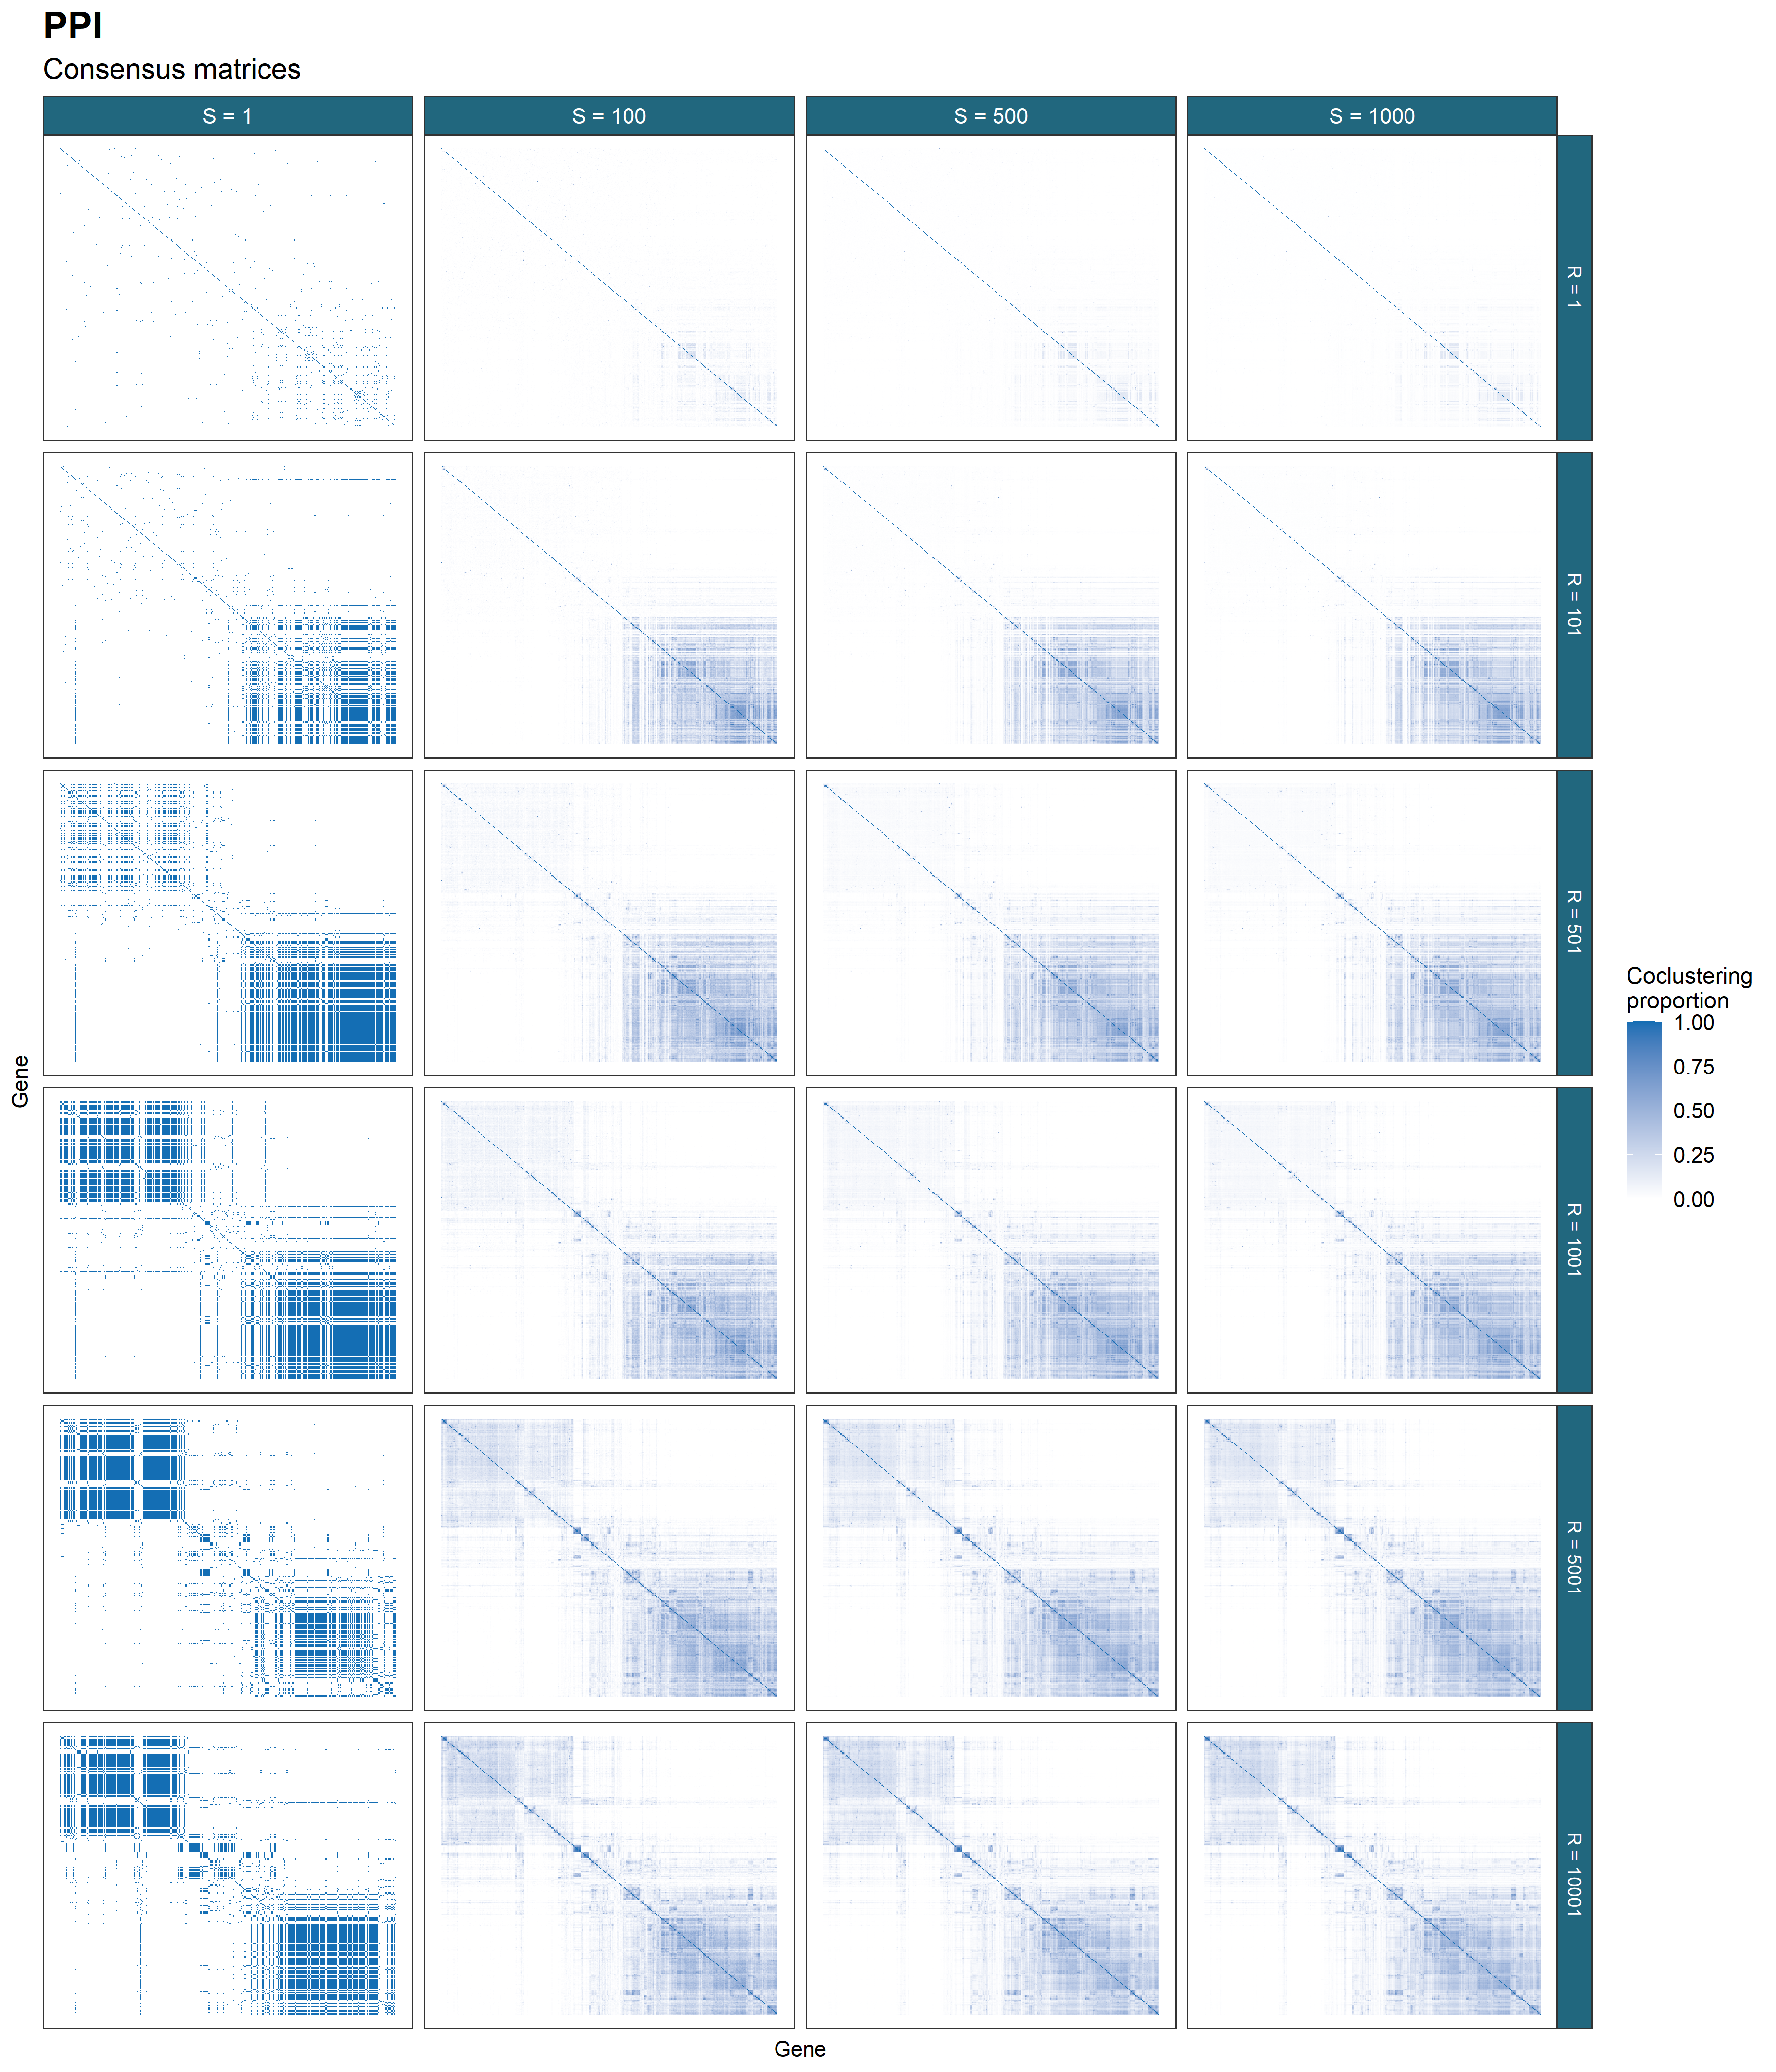
\includegraphics[scale=0.8]{../Images/Yeast/PPICMcomparison.png}
	\caption{The PPI dataset has awkward characteristics for modelling. A wide, sparse dataset it is again chain depth that is the most important parameter for the ensemble. Similar to the results in figure \ref{fig:chipchipCMs}, the matrices only stabilise from $R=5001$ to $R=10001$.}
	\label{fig:ppiCMs}
\end{figure}

If we compare the distribution of sampled values for the $\phi$ parameters for the Bayesian chains that we keep based upon their convergence diagnostics, the final ensemble used ($R=10001$, $S=1000$) and the pooled samples from the 5 long chains, then we see that the ensemble consisting of the long chains (which might be believed to sampling different parts of the posterior distribution) is closer in its appearance to the distributions sampled by the Consensus clustering than to any single chain.

\begin{figure}
	\centering
	\includegraphics[scale=0.6]{../Images/Yeast/ComparisonDensities.png}
	\caption{The sampled values for the $\phi$ parameters from the long chains, their pooled samples and the consensus using 1000 chains of depth 10,001. The long chains display a variety of behaviours. Across chains there is no clear consensus on the nature of the posterior distribution. The samples from any single chain are not particularly close to the behaviour of the pooled samples across all three parameters. It is the Consensus clustering that most approaches this pooled behaviour.}
	\label{fig:densityComparison}
\end{figure}

\subsection{GO term over-representation} \label{sec:goTermOverRep}
To validate our analysis we test if the predicted clusters have a higher concentration of specific  Gene Ontology (GO) terms than would be expected by chance, conditioning on the background set of the 551 yeast genes in the data. The \texttt{Bioconductor} packages \texttt{clusterProfiler} \citep{yu2012clusterProfiler}, \texttt{biomaRt} \citep{durinck2009mapping} and the annotation package \texttt{org.Sc.sgd.db} \citep{carlson2014org} were used. Clusters were predicted from the Posterior similarity matrices of the chains kept from section \ref{sec:bayesianConvergence} and the consensus matrix of the largest ensemble run (i.e. $CC(10001, 1000)$). The gene labelled YIL167W was not found in the annotation database and was dropped from the analysis leaving a background universe of 550 genes. A hypergeometric test was used to check if the number of genes associated with specific GO terms within a cluster was greater than expected by random given the 550 possible genes. The false discovery rate of this test was controlled using the Benjamini-Hochberg correction \citep{benjamini1995controlling} and significance threshold of 0.05 was used. The over-represented GO terms were then plotted to compare methods. The three different ontologies of "Molecular function" (\textbf{MF}), "Biological process" (\textbf{BP}) and "Cellular component" (\textbf{CC}) were all investigated.

\begin{figure}
	\centering
	\includegraphics[scale=0.6]{../Images/Yeast/ComparisonDensities.png}
	\caption{.}
	\label{fig:yeastGOMF}
\end{figure}



%\bibliographystyle{natbib}
\bibliographystyle{plainnat}
\bibliography{consensusClusteringAnalysis}  

\end{document}
